% =============================================================================
%  CSD Assignment 1 — Phase 3 Final Report
%  NOTE: the course requires the official Overleaf template. Copy each \section
%  below into the matching section of that template (do not change its formatting).
%  Items marked \todo{...} must be filled in with values measured on the lab systems.
% =============================================================================
\documentclass[11pt,a4paper]{article}
\usepackage[margin=2.2cm]{geometry}
\usepackage{amsmath,booktabs,graphicx,hyperref,xcolor,listings,tikz,float,caption}
\usetikzlibrary{positioning,arrows.meta,fit}
\newcommand{\todo}[1]{\textcolor{red}{\textbf{[TODO: #1]}}}
\lstset{basicstyle=\ttfamily\footnotesize,breaklines=true,frame=single,columns=fullflexible}
\graphicspath{{figures/}}

\title{Pond Site \& Catchment Planner\\\large CSD Assignment 1 --- Phase 3 Final Report}
\author{Ranga Chandra Naga Venkata Chaitanya Kumar \quad (Roll No.\ 12341740)}
\date{}

\begin{document}
\maketitle

\begin{center}
\begin{tabular}{ll}
\textbf{GitHub repository} & \url{https://github.com/chaitanyakumarAI/Pond_catchment_analysis} \\
\textbf{Front-end URL} & \url{http://10.1.75.51:5237/} \todo{confirm after deployment}\\
\textbf{Demo video} & \todo{YouTube link}\\
\end{tabular}
\end{center}

% -----------------------------------------------------------------------------
\section{Problem Statement}
Small farm ponds harvest monsoon runoff for irrigation. Choosing where to dig one
needs three answers for a given piece of land: \emph{where} the pond should go,
\emph{which area drains into it} (its catchment) and \emph{how much water} that
catchment can deliver in a year. The goal of this assignment is a fast, working web
system in which a user selects a land area on a map and immediately sees the
suggested pond location, the catchment area and the expected water volume overlaid
on the map. The system has to run on the four lab systems provided and must handle
concurrent users gracefully.

% -----------------------------------------------------------------------------
\section{Requirements}
\textbf{Functional.}
(F1) A working front-end with an interactive map;
(F2) selection of a land area on the map (rectangle or free polygon);
(F3) results computed only for the selected area;
(F4) results include pond location, catchment area and expected annual water volume;
(F5) all three are drawn on the map;
(F6) optional upload of the user's own KML/KMZ contour map (Phase 1 compatibility).

\textbf{Non-functional.}
(N1) Interactive latency: an area query should return in well under one second;
(N2) horizontal scaling over the four lab systems with no single worker as a bottleneck;
(N3) graceful behaviour under overload (bounded queueing and explicit shedding rather than timeouts);
(N4) fault tolerance: loss of a worker must not fail user requests;
(N5) input validation with clear messages (area too small or large, outside the data, bad parameters).

% -----------------------------------------------------------------------------
\section{System Architecture}
\begin{figure}[H]
\centering
\resizebox{\linewidth}{!}{%
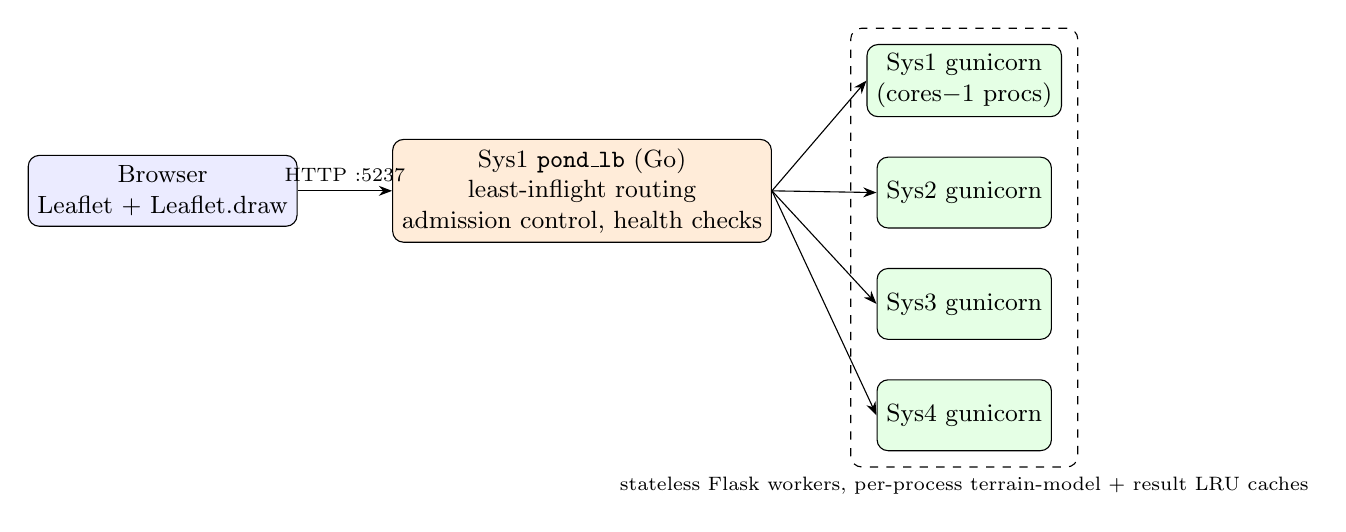
\begin{tikzpicture}[node distance=5mm and 12mm,
  box/.style={draw,rounded corners,align=center,minimum height=9mm,font=\small,fill=#1},
  box/.default=white, >=Stealth]
\node[box=blue!8] (br) {Browser\\Leaflet + Leaflet.draw};
\node[box=orange!15,right=of br] (lb) {Sys1 \texttt{pond\_lb} (Go)\\least-inflight routing\\admission control, health checks};
\node[box=green!10,right=of lb,yshift=14mm] (w1) {Sys1 gunicorn\\(cores$-$1 procs)};
\node[box=green!10,below=of w1] (w2) {Sys2 gunicorn};
\node[box=green!10,below=of w2] (w3) {Sys3 gunicorn};
\node[box=green!10,below=of w3] (w4) {Sys4 gunicorn};
\draw[->] (br) -- node[above,font=\scriptsize]{HTTP :5237} (lb);
\foreach \w in {w1,w2,w3,w4} \draw[->] (lb.east) -- (\w.west);
\node[draw,dashed,rounded corners,fit=(w1)(w4),inner sep=2mm,label={[font=\scriptsize]below:stateless Flask workers, per-process terrain-model + result LRU caches}] {};
\end{tikzpicture}}
\caption{Deployment on the four lab systems. Every request carries its dataset and polygon, so any worker can serve it.}
\end{figure}

\textbf{Front-end.} A single-page Leaflet application with satellite, topographic and
street base maps. The user draws a rectangle or polygon (Leaflet.draw) inside the
dashed data-coverage boundary. The analysis runs automatically once the shape is
complete. Rainfall, runoff coefficient and pond depth can be edited. Results are drawn
as the selected-area outline, one coloured catchment polygon per pond, a blue pond
footprint to scale and a label per site giving the water volume, catchment area and
pond capacity. Terrain plots and a rotatable 3D model are available for the same
selection. Leaflet, Leaflet.draw and Plotly are served from the application itself, so
the page does not depend on external CDNs.

\textbf{API.} \texttt{POST /api/analyzeArea} takes
\texttt{\{polygon, rainfall\_mm, runoff\_coeff, pond\_depth\_m\}} as JSON, or as
multipart data together with a KML/KMZ file. It returns JSON with the pond sites, the
catchments, the volumes and a GeoJSON \texttt{FeatureCollection} whose features are
typed \texttt{pond\_site}, \texttt{catchment}, \texttt{pond\_footprint} and
\texttt{selected\_area}. The Phase~1 routes (\texttt{/analyzeContour},
\texttt{/findCatchment}, \texttt{/api/sample}) are unchanged. \texttt{/api/coverage},
\texttt{/health}, \texttt{/metrics} and \texttt{/lb/stats} support the UI and
operations.

\textbf{Stateless workers.} Phase~1 kept the last result in a process-global variable,
so the plot routes only worked if the same process served the follow-up request. That
breaks behind a load balancer. In Phase~3 every request carries the dataset (the sample
map id, or the uploaded file) and the polygon. A worker that has no cached result simply
recomputes it, because the pipeline is deterministic. No sticky sessions or shared
store are needed.

% -----------------------------------------------------------------------------
\section{Algorithm}
The pipeline is split into two stages. Stage~A depends only on the terrain, is
computed once per dataset and is cached. Stage~B depends on the user's selection and
takes only milliseconds.

\subsection*{Stage A --- terrain and hydrology model (once per dataset)}
\begin{enumerate}\itemsep0pt
\item \textbf{Parsing.} Contour vertices $(\lambda,\varphi,z)$ are read from KML/KMZ
      (160\,473 vertices on 2\,711 contour lines in the sample). Spike vertices are removed
      with a percentile window $[P_{0.5}-\Delta, P_{99.5}+\Delta]$, where $\Delta = \tfrac12(P_{99.5}-P_{0.5})$,
      so no fixed elevation constants are needed.
\item \textbf{Projection.} The data are projected to the local UTM zone, chosen
      automatically (EPSG:32644 for the sample), so that distances and areas are in metres.
\item \textbf{DEM.} Linear interpolation (with nearest-neighbour fill) onto a
      $200\times161$ grid (16.2\,m cells), then Gaussian smoothing with $\sigma=1$.
\item \textbf{Sink filling.} Priority-Flood (Barnes, 2014) fills the pits. The depression depth is
      $d = z_{\text{filled}} - z_{\text{raw}}$, which marks natural water-retention basins.
\item \textbf{Slope and flow.} Horn's 3$\times$3 slope. D8 flow direction (steepest
      descent to one of the eight neighbours). Flow accumulation $A$ is computed by processing cells from high to low.
\item \textbf{River corridor.} A cell is treated as river if $A \ge P_{95}(A)$, or if it lies in the lowest 18\,\% of elevations with a slope below $3^\circ$.
      A Euclidean distance transform gives each cell's distance to the river. Pond sites must lie at least
      $\max(120\text{ m}, 0.25\,d_{\max})$ from the river (flood safety).
\item \textbf{Suitability.} $\text{TWI}=\ln(a/\tan\beta)$, and
\[ \text{PSI} = 0.35\,\hat d + 0.30\,\widehat{\ln(1{+}A)} + 0.20\,\widehat{\text{TWI}} + 0.15\,(1-\hat z), \]
      where $\hat{\cdot}$ denotes min--max normalisation. Only cells with slope in $[0.3^\circ, 8^\circ)$ and $d>0$ are eligible.
\end{enumerate}

\subsection*{Stage B --- area query (per request)}
\begin{enumerate}\itemsep0pt
\item \textbf{Validation.} The polygon is projected to UTM and intersected with the
      convex hull of the data. It is rejected (HTTP 422) if it is smaller than 0.5\,ha, larger than 50\,km$^2$, or less
      than 60\,\% covered by contour data.
\item \textbf{Rasterisation.} The polygon is rasterised onto the model grid. PSI is set to zero
      outside it. If a small parcel has fewer than 20 eligible cells, the river buffer is relaxed in steps
      (120$\to$90$\to$60$\to$30$\to$0\,m), and the step used is reported.
\item \textbf{Site selection.} PSI local maxima ($16\times16$ window) are ranked. A site is kept if
      its upstream area is at least 1\,ha and it lies at least 350\,m from the sites already kept. At most four sites are returned.
\item \textbf{Catchment.} For each site, a reverse-D8 traversal collects every upstream
      non-river cell. The true hydrological catchment is kept even where it extends beyond
      the parcel boundary, and the part inside the parcel is reported separately. The polygon
      is the union of the cells, buffered and simplified with Shapely.
\item \textbf{Water volume.} The rational method gives
      $Q = C\cdot P\cdot A$ (default $C=0.35$, $P=850$\,mm). The recommended capacity is
      $\min(0.18\,Q,\;25\,000\,\text{m}^3)$, and the square footprint has side
      $\sqrt{\text{capacity}/\text{depth}}$. A stage--storage curve from the DEM gives the natural storage of the basin at 0.5--3\,m depths.
\end{enumerate}
Stage~B only reads the cached arrays, so its cost is proportional to the number of
cells in the parcel and its catchments rather than to the whole map.

% -----------------------------------------------------------------------------
\section{Results}
\begin{figure}[H]
\centering
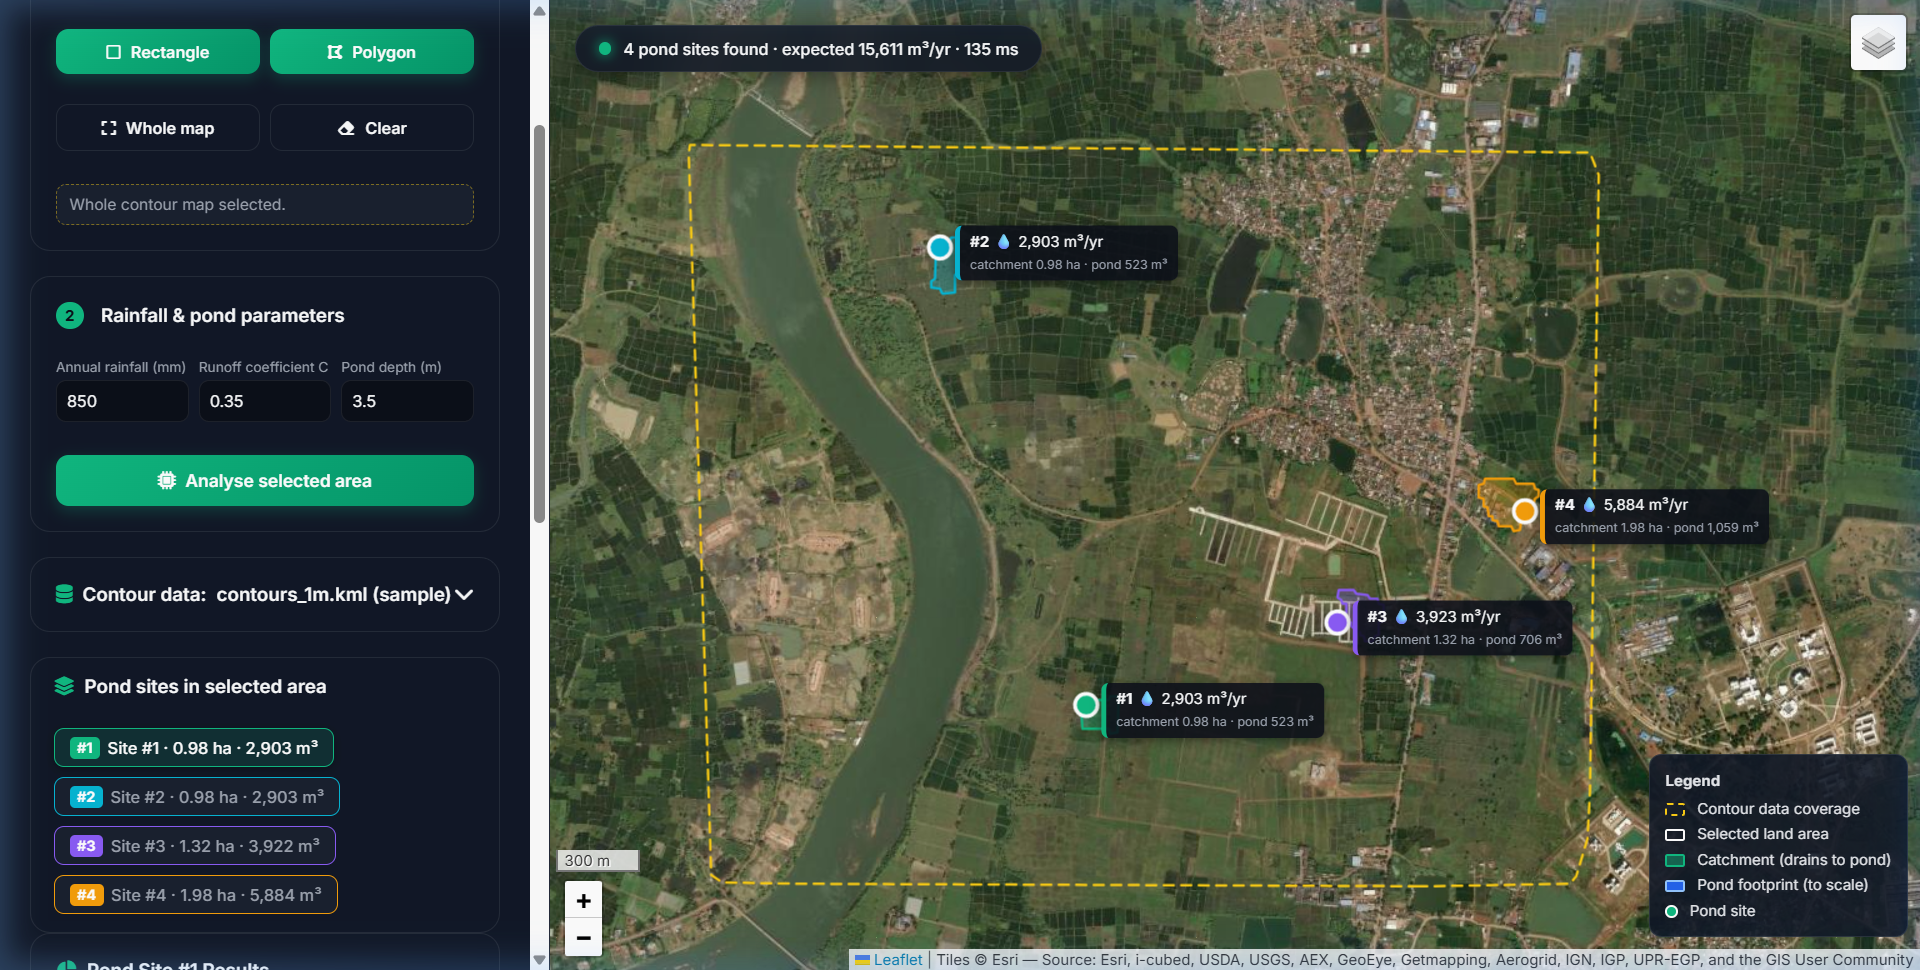
\includegraphics[width=\linewidth]{ui_result.png}
\caption{A polygon drawn on the sample map returns four pond sites, their catchments and
their annual volumes (14\,199\,m$^3$/yr in total) in 45\,ms. The dashed yellow line is the
data coverage. \todo{replace with a screenshot taken on the lab deployment; the base-map tiles were blocked in the build sandbox}}
\end{figure}

\begin{table}[H]
\centering\small
\resizebox{\linewidth}{!}{%
\begin{tabular}{lrrrrrr}
\toprule
Selected area & Area (ha) & Sites & Top-site catchment (ha) & Top-site $Q$ (m$^3$/yr) & All sites $Q$ (m$^3$/yr) & Stage-B time \\
\midrule
A: west half (rectangle)    & 418.3 & 3 & 0.98 & 2\,903 & 9\,022  & 21 ms \\
B: east half (rectangle)    & 418.3 & 4 & 1.32 & 3\,922 & 17\,651 & 35 ms \\
C: 1\,km block (rectangle)  & 103.4 & 2 & 0.98 & 2\,903 & 7\,374  & 15 ms \\
D: triangle (polygon)       & 189.5 & 2 & 0.98 & 2\,903 & 7\,374  & 15 ms \\
E: 10\,ha field             & 10.3  & 1 & 0.98 & 2\,903 & 2\,903  & 7 ms \\
Whole map                   & ---   & 4 & 0.98 & 2\,903 & 15\,611 & 29 ms \\
\bottomrule
\end{tabular}}
\caption{Area queries on \texttt{contours\_1m.kml} ($P=850$\,mm, $C=0.35$). The top
site at 21.245616\,N, 81.295040\,E (elevation 282.8\,m, 167\,m from the river,
recommended pond 12.2$\times$12.2$\times$3.5\,m, 522\,m$^3$) is identical to the Phase~1
whole-map result, which confirms that Stage~B is consistent with it. Times are the median of five runs on one core.}
\end{table}

\begin{figure}[H]
\centering
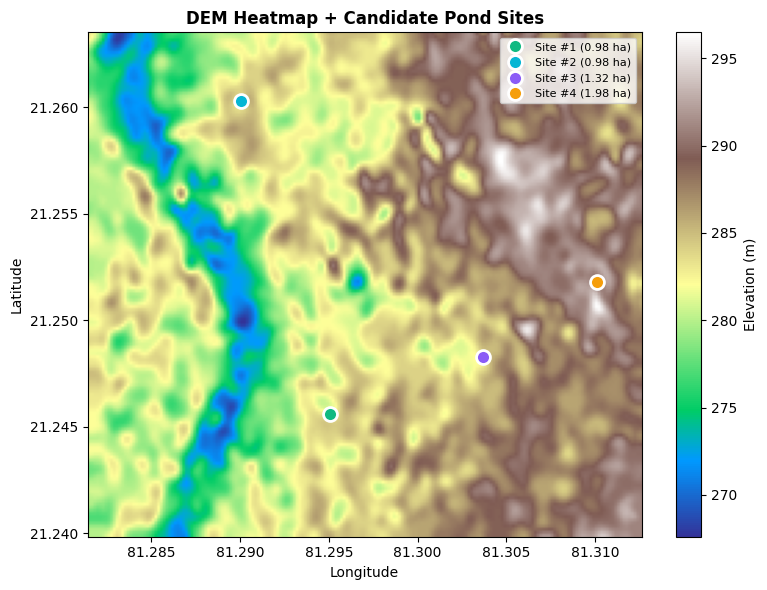
\includegraphics[width=0.49\linewidth]{dem_heatmap.png}\hfill
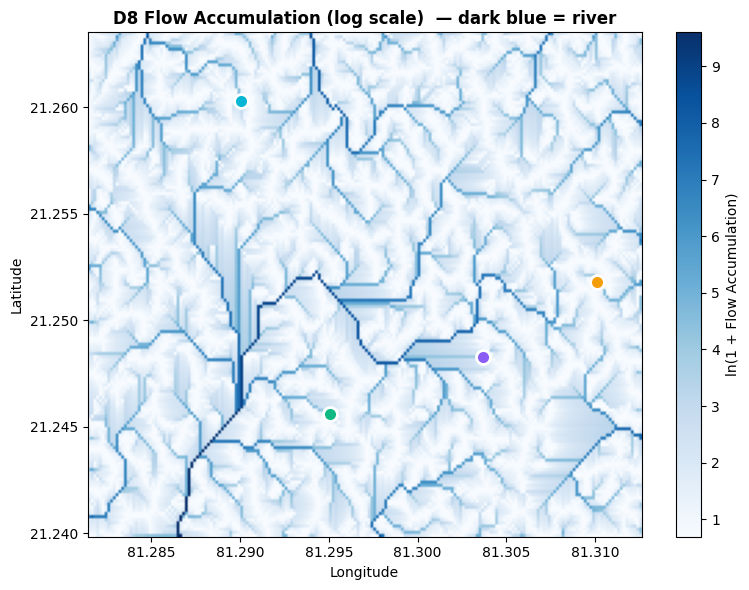
\includegraphics[width=0.49\linewidth]{flow_accumulation.png}
\caption{Interpolated DEM with candidate sites (left) and D8 flow accumulation (right). The
river valley on the west side is excluded by the river-corridor buffer.}
\end{figure}

% -----------------------------------------------------------------------------
\section{Performance, Scaling and System Limitations}
\textbf{Cost profile} (measured on one core of a 2-vCPU VM):
parsing 0.39\,s, Stage~A model 0.50\,s (once per dataset per process),
Stage~B area query 7--35\,ms, a result-cache hit about 0.2\,ms, an uploaded 6.4\,MB KML about 1.0\,s
on first use, the six terrain plots about 3.5\,s. The work is CPU-bound (numpy, scipy),
so the unit of capacity is a CPU core.

\textbf{Design decisions for scale.}
\begin{itemize}\itemsep0pt
\item \emph{Pre-computation and caching}: the sample model is built at start-up with
      \texttt{gunicorn --preload}, so worker processes share it copy-on-write. Uploaded datasets are cached by the
      SHA-1 of their bytes (LRU of 4 models, each about 5\,MB). Results are cached by
      SHA-1 of (dataset, polygon, parameters) (LRU of 256).
\item \emph{Process model}: gunicorn sync workers, one per core on Sys2--4 and cores$-$1 on
      Sys1, which also runs the load balancer. \texttt{max\_requests} recycles workers so memory stays bounded.
\item \emph{Load balancer} (\texttt{cluster/pond\_lb.go}, written for this assignment):
      least-outstanding-requests routing, round-robin among equally loaded backends, and a
      switch away from a node only when its EWMA latency is clearly worse. The per-node
      concurrency cap equals its worker count. Excess requests wait in a bounded
      queue (15\,s) and are then \emph{shed} with \texttt{503 + Retry-After}, so overload
      produces fast explicit errors instead of a timeout storm. Health is checked
      actively every 2\,s and failed nodes are also ejected passively. Request bodies are buffered so that a
      connection failure is retried once on another node.
\item \emph{Limits enforced}: uploads up to 25\,MB, polygons with 3--500 vertices and an area of 0.5\,ha--50\,km$^2$
      with at least 60\,\% data coverage, and parameters inside physical ranges. The upload is sub-sampled to at most
      12\,000 vertices, which bounds interpolation time whatever the file size.
\end{itemize}

\textbf{Stress test.} \texttt{cluster/locustfile.py} models the traffic mix: 60\,\% new
parcels, 20\,\% popular (cached) parcels, 10\,\% whole-map queries, 5\,\% page loads and 5\,\% 3D meshes.
\texttt{cluster/run\_stress.py} steps the number of users and records throughput, p50/p95/p99 latency and errors.

\begin{table}[H]
\centering\small
\begin{tabular}{rrrrrrr}
\toprule
Users & \multicolumn{3}{c}{1 worker (direct)} & \multicolumn{3}{c}{4 workers via \texttt{pond\_lb}} \\
      & req/s & p95 (ms) & err \% & req/s & p95 (ms) & err \% \\
\midrule
10  & 8.2  & 34  & 0 & 8.4  & 32  & 0 \\
50  & 40.4 & 60  & 0 & 41.1 & 37  & 0 \\
150 & 101.1 & 550 & 0 & 121.0 & 100 & 0 \\
\bottomrule
\end{tabular}
\caption{Local dry run: four single-process workers and the LB on one 2-vCPU VM, with Locust
on the same machine. At 150 users the load balancer cuts p95 latency from 550 to 100\,ms.
Throughput is limited by the VM's two cores and is not representative of the lab cluster.
\todo{replace with \texttt{results/stress\_summary.csv} from the 4-system run}}
\end{table}

\begin{figure}[H]
\centering
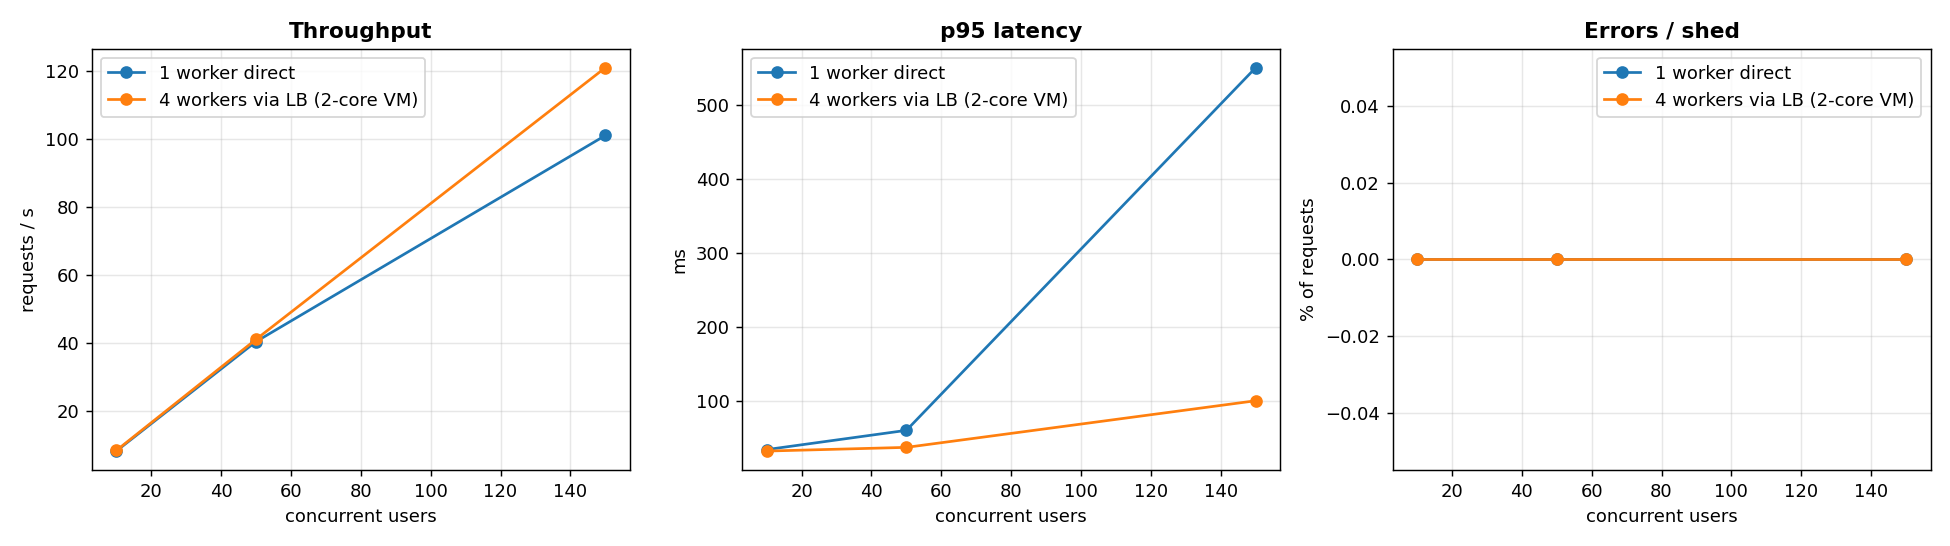
\includegraphics[width=\linewidth]{local_dryrun_plot.png}
\caption{Throughput, p95 latency and error rate against concurrent users (local dry run). \todo{replace with the lab plot}}
\end{figure}

\textbf{Fault tolerance (verified).} Killing one of the four workers during a request
stream produced zero failed requests. The LB marked the node unhealthy and re-routed
traffic, then re-admitted it after restart. Sixteen concurrent plot requests on a saturated
cluster were answered with 3 successes and 13 immediate 503s, which is the intended shedding behaviour.

\textbf{Capacity estimate.} With $N$ cores in total and a mean service time $S$, the peak
throughput is about $N/S$. For new-parcel queries ($S\approx$ 25--40\,ms including JSON serialisation), each core
serves about 25--40 requests/s, so the four systems give roughly \todo{total cores}$\times$30 requests/s before the LB starts queueing.
The terrain plots are about 100 times heavier (3.5\,s) and are the first to be shed.

\textbf{Known limitations.} (i) Caches are per process, so a newly uploaded file is modelled
once on each node that sees it; consistent hashing on the dataset id would remove this. (ii)
The single LB on Sys1 is a single point of failure; a keepalived VIP or DNS round-robin
over two LBs would remove it. (iii) The runoff model uses one annual $C$ and $P$ rather
than event-based SCS-CN, and it does not model soil infiltration or evaporation. (iv) DEM resolution is
limited by the contour interval (1\,m) and the 200-column grid, so parcels smaller than about 0.5\,ha are rejected.

% -----------------------------------------------------------------------------
\section{Testing}
\texttt{test\_api.py} checks health, coverage, area analysis (all four GeoJSON
feature kinds present), rejection of an out-of-coverage area (422), the Phase~1 upload
route and the 3D mesh. It passed against the local cluster. The front-end was tested with a headless
Chromium (Playwright) script that draws rectangles and polygons, reads the rendered results and opens
the plot and 3D views. The Phase~1 whole-map output is reproduced exactly (same four
sites and values), which confirms that the refactor preserved behaviour.

% -----------------------------------------------------------------------------
\section{Conclusion}
The system meets every Phase~3 requirement. The user draws a land area, and within
tens of milliseconds sees where to dig the pond, which area drains into it and how much
water it will collect, all on the map. Splitting the pipeline into a cached terrain
model and a cheap area query is what makes it fast. Stateless workers behind an
admission-controlled load balancer let it use all four lab systems and degrade
predictably under overload.

% -----------------------------------------------------------------------------
\appendix
\section{API example}
\begin{lstlisting}
curl -X POST http://10.1.75.51:5237/api/analyzeArea -H "Content-Type: application/json" \
 -d '{"polygon":[[81.29,21.245],[81.30,21.245],[81.30,21.254],[81.29,21.254],[81.29,21.245]],
      "rainfall_mm":850,"runoff_coeff":0.35,"pond_depth_m":3.5}'
# -> {"success":true,"served_by":"sys3","cache_hit":false,"data":{"pond_location":{...},
#     "catchment_summary":{"area_hectares":0.98,...},"expected_water_volume_m3":2902.62,
#     "all_candidate_sites":[...],"selected_area":{...},"geojson_layers":{...}}}
\end{lstlisting}

\section{Deployment}
\begin{lstlisting}
cd cluster && GOOS=linux GOARCH=amd64 go build -o pond_lb . && cd ..
python cluster/deploy_cluster.py      # uploads code, starts gunicorn on Sys1-4 and pond_lb on Sys1
python cluster/deploy_cluster.py --status
python cluster/run_stress.py --target cluster=http://10.1.75.51:5237 --users 10 50 100 200
\end{lstlisting}
\end{document}
